	\section{Análisis Cinemático del brazo}
	\subsection{Modelo Cinemático Directo}
	\subsubsection{Parámetros y estudio del MCD según Denavit-Hartemberg}
	Uno de los modos de estudio del problema cinemático directo de un robot es el procedimiento de Denavit-Hartemberg, el cual se basa en la realización de cambios de sistema de referencia empleando las matrices de transformación homogéneas. Siguiendo una serie de pasos, se llegará a obtener los siguientes parámetros que definen la cinemática directa del robot.\\
Por tanto, los sistemas de referencia definidos se muestran a continuación:
	% %%%%%%%%%%%%%%%%%
	% anadir foto del analisis del brazo
	% %%%%%%%%%%%%%%%%%
	\begin{figure}[h!]
		\centering
		\includegraphics[width=.5\textwidth]{ejes_DH}
		\caption{Sistemas de referencia definidos}
	\end{figure}

En base a esos sistemas de referencia, los parámetros de Denavit-Hartemberg obtenidos serán:
%Tabla de Denavit-Hartenberg
\begin{center}
	\begin{tabular}{|c||c|c|c|c|}
		\hline
		Articulación & $\theta_{i}$ & $d_{i}$ & $a_{i}$ & $\alpha_{i}$ \\
		\hline
		1 & $\theta_{1}$     				 &   L0+L1    &  			0 			 &  $\frac{\pi}{2}$  \\
		\hline
		2 & $\theta_{2}$ 				 &    0     &L2 & 0  \\
		\hline
		3 & $\theta_{3}$ &    L3    & 			 L2			 &  0\\
		\hline
	\end{tabular}
\end{center}

	\subsubsection{Matrices de transformación homogéneas del robot}
	A continuación, se mostrarán las matrices de transformación homogéneas que definen los cambios de sistema de referencia que han hecho posible relacionar el sistema de referencia base con el del efector final. La matriz de transformación homogénea que relaciona un sistema de referencia con el siguiente se define como:\\
	\begin{equation}
	{^{i-1}}A_{i}=Rotz(\theta_{i})*T(0,0,d_{i})*T(d_{i},0,0)*Rotx(\alpha_{i})=
	\begin{pmatrix}
	cos(\theta_{i}) & -sin(\alpha_{i})cos(\theta_{i})	& sin(\alpha_{i})sin(\theta_{i})  & a_{i}cos(\theta_{i})     \\
	sin(\theta_{i}) &  sin(\alpha_{i})cos(\theta_{i})	& -sin(\alpha_{i})cos(\theta_{i}) & a_{i}sin(\theta_{i})     \\
	0 		&  			sin(\alpha_{i})   		& 		cos(\alpha_{i})			  & d_{i}\\
	0 		&					0				&				0  		  		  & 1
	\end{pmatrix}
	\end{equation}

	Ahora que se ha definido la matriz general, se definirán las matrices de transformación homogéneas de cada cambio de sistema de referencia del robot: \\

	\[ {^0}A_{1} =
	\left( \begin{array}{cccc}
	cos(\theta_{1}) &  0 &  sin(\theta_{1}) & 0  \\
	sin(\theta_{1}) &  0 & -cos(\theta_{1}) & 0  \\
	0		&  1 &		 0 			& L0+L1 \\
	0		&  0 & 		 0			& 1
	\end{array} \right) \]

	\[ {^1}A_{2} =
	\left( \begin{array}{cccc}
	cos(\theta_{2}) & -sin(\theta_{2}) & 0 & L2cos(\theta_{2}) \\
	sin(\theta_{2}) & cos(\theta_{2})  & 0 & L2sin(\theta_{2})  \\
	0 		 	   & 			0 			& 1	& 		0 			 \\
	0		 	   &			 0			& 0	& 		1
	\end{array} \right) \]

	\[ {^2}A_{3} =
	\left( \begin{array}{cccc}
	cos(\theta_{3}) &  -sin(\theta_{3}) &  0 & L3cos(\theta_{3})   \\
	sin(\theta_{3}) &  cos(\theta_{3}) &  0 & L3sin(\theta_{3})   \\
	0 					 &  0 &  				1 					  & 0 \\
	0 					 &  0 & 				 0					  & 1
	\end{array} \right) \]

	\subsubsection{Ecuaciones simbólicas del MCD}
	A partir de estos parámetros será posible obtener las matrices de transformación homogéneas asociadas a cada traslación y giro de sistema de referencia. Si se premultiplican las matrices desde la base hasta el punto final del brazo (efector final), la matriz de transformación obtenida será:
	\begin{equation}
	{^3}T_{0} =
	\left( \begin{array}{cccc}
	cos(\theta_{2}+\theta_{3})cos(\theta_{1})  & -sin(\theta_{2}+\theta_{3})cos(\theta_{1}) &  -sin(\theta_{1})  & cos(\theta_{1})[L3cos(\theta_{2}+\theta_{3}) + L2cos(\theta_{2})] \\
	cos(\theta_{2}+\theta_{3})sin(\theta_{1})  & -sin(\theta_{2}+\theta_{3})sin(\theta_{1}) & cos(\theta_{1})  & sin(\theta_{1})[L3cos(\theta_{2}+\theta_{3}) + L2cos(\theta_{2})] \\
	sin(\theta_{2}+\theta_{3})		 		  &		 cos(\theta_{2}+\theta_{3})		        & 		0 			& L0 + L1 + L3sin(\theta_{2}+\theta_{3}) + L2sin(\theta_{2})	 \\
	0						  &		 	0  									&       0		    &   1
	\end{array} \right)
	\end{equation}
	Donde se puede extraer que la matriz de orientación del efector final y la posición del mismo respecto al sistema de referencia de la base son:
	\[ noa =
	\left( \begin{array}{ccc}
cos(\theta_{2}+\theta_{3})cos(\theta_{1})  & -sin(\theta_{2}+\theta_{3})cos(\theta_{1}) & -sin(\theta_{1})  \\
cos(\theta_{2}+\theta_{3})sin(\theta_{1})  & -sin(\theta_{2}+\theta_{3})sin(\theta_{1}) & cos(\theta_{1})  \\
sin(\theta_{2}+\theta_{3})		 		  &		 cos(\theta_{2}+\theta_{3})		        & 		0
	\end{array} \right) \]

	\[ p =
	\left( \begin{array}{c}
	cos(\theta_{1})[L3cos(\theta_{2}+\theta_{3}) + L2cos(\theta_{2})] \\
	sin(\theta_{1})[L3cos(\theta_{2}+\theta_{3}) + L2cos(\theta_{2})] \\
	L0 + L1 + L3sin(\theta_{2}+\theta_{3}) + L2sin(\theta_{2})
	\end{array} \right) \]

	\subsection{Modelo Cinemático Inverso}

	En lo que a la resolución del modelo cinemático inverso del robot respecta, se basará en obtener los valores de las variables articulares a partir de la posición del efector final. Por tanto, se partirá de las ecuaciones del vector $p$:

	\begin{center}
		$px=cos(\theta_{1})[L3cos(\theta_{2}+\theta_{3}) + L2cos(\theta_{2})]$ \\
		$py=sin(\theta_{1})[L3cos(\theta_{2}+\theta_{3}) + L2cos(\theta_{2})]$ \\
		$pz=L0 + L1 + L3sin(\theta_{2}+\theta_{3}) + L2sin(\theta_{2})$
	\end{center}

	Para obtener las ecuaciones que definen el valor de $\theta_{1}$,$\theta_{2}$ y $\theta_{3}$, se trabajará con las funciones que definen px,py y pz. Será necesario definir los ángulos empleando la función atan2 de \textit{Matlab}, ya que de ese modo se distinguirá en qué cuadrante se encuentra la tangente.\\
	Por tanto el objetivo es obtener el valor del seno y el coseno de cada ángulo.\\

	Se comenzará obteniendo el valor de $\theta_{1}$. Para ello se define:\\
	\begin{center}
		$ A = \sqrt{px^{2}+py^{2}} = L3cos(\theta_{2}+\theta_{3}) + L2cos(\theta_{2})$
	\end{center}
	de ese modo, se obtiene $\theta_{1}$ como:\\
	\begin{equation}
	\theta_{1}=atan2(sin(\theta_{1}),cos(\theta_{1}))=atan2(\frac{py}{A},\frac{px}{A})
	\end{equation}
	Para obtener el valor de $\theta_{3}$, se comenzará a partir de pz y, se definirá la siguiente variable auxiliar:\\
	\begin{center}
		$ B=pz-L1-L0=L3sin(\theta_{2}+\theta_{3}) + L2sin(\theta_{2})$
	\end{center}
	Si se trabaja con las dos variables auxiliares creadas, A y B, y se crea la nueva variable C, se conseguirá obtener el valor del ángulo deseado:\\
	\begin{center}
		$C= A^{2} + B^{2} = L2^{2}+ 2L2L3cos(\theta_{3}) + L3^{2} $
	\end{center}

	Cómo último paso para obtener el valor de $\theta_{3}$, se despejará el valor del coseno del mismo:\\
	\begin{center}
		$ (cos(\theta_{3})) = \frac{C-L2^{2}-L3^{2}}{2L2L3} $
	\end{center}
	Por tanto, $\theta_{3}$ se define como:\\
	\begin{equation}
	\theta_{3}=\beta -atan2(sin(\theta_{3}),cos(\theta_{3}))=\beta-atan2(\pm \sqrt{1-(\frac{C-L2^{2}-L3^{2}}{2L2L3})^{2}},\frac{C-L2^{2}-L3^{2}}{2L2L3} )
	\end{equation}

	Por último, se hallará el valor de la variable articular $\theta_{2}$. Para ello, se partirá de la ecuación A y se desarrollará empleando la fórmula del coseno del ángulo doble. La ecuación quedará de la forma: \\
	\begin{center}
		$A=L3cos(\theta_{2}+\theta_{3})+L2cos(\theta_{2})=L3[cos(\theta_{2})cos(\theta_{3})-sin(\theta_{2})sin(\theta_{3})]+L2cos(\theta_{2})=$\\ \vspace{0.3cm} $L3cos(\theta_{2})cos(\theta_{3})-L3sin(\theta_{2})sin(\theta_{3})+L2cos(\theta_{2})$
	\end{center}
donde será de ayuda despejar la función A en una suma de un término por el seno de $ \theta_{2}$ y otro término por el coseno del mismo ángulo. De ese modo será posible intentar obtener dicho ángulo empleando un cambio a coordenadas polares:
	\begin{center}
		$A=cos(\theta_{2})[L3cos(\theta_{3})+L2]-sin(\theta_{2})[L3sin(\theta_{3})]$\\
		\vspace{0.3cm}
		\fbox{%
			\begin{minipage}[b][1.2cm][c]{0.9\textwidth}
				$\rho cos(\alpha)=L3cos(\theta_{3})+L2$ \hspace*{3cm} $\rho=\sqrt{(L3sin(\theta_{3}))^{2}+(L3cos(\theta_{3})+L2)^{2}} $\\
				$\rho sin(\alpha)=L3sin(\theta_{3})$ \hspace*{3.8cm} $\alpha=atan2(L3sin(\theta_{3}),L3cos(\theta_{3})+L2)$\\
			\end{minipage}
		}\hfill
	\end{center}
	Sustituyendo en la ecuación A y empleando la fórmula del coseno del ángulo suma, se podría definir:\\
	\begin{center}
	$A=\rho cos(\theta_{2})cos(\alpha)-\rho sin(\theta_{2})sin(\alpha)$ $\rightarrow$ $A=\rho cos(\theta_{2}+\alpha)$
	\end{center}

	Despejando el valor del coseno $\theta_{3}$ se obtendrá:
	\begin{equation}
	\theta_{2}=atan2(\pm \sqrt{1-(\frac{A}{\rho})^{2}},\frac{A}{\rho})-\alpha
	\end{equation}
	De ese modo, la solución del problema cinemático inverso está formada por siguientes ecuaciones:
	\begin{center}
		$\theta_{1}=atan2(sin(\theta_{1}),cos(\theta_{1}))=atan2(\frac{py}{A},\frac{px}{A})$ \\
		$\theta_{2}=atan2(\pm \sqrt{1-(\frac{A}{\rho})^{2}},\frac{A}{\rho})-\alpha$ \\
		$\theta_{3}=\beta -atan2(sin(\theta_{3}),cos(\theta_{3}))=\beta-atan2(\pm \sqrt{1-(\frac{C-L2^{2}-L3^{2}}{2L2L3})^{2}},\frac{C-L2^{2}-L3^{2}}{2L2L3} )$
	\end{center}

	\subsection{Jacobiano del robot y análisis de puntos singulares}
Aunque éste apartado no cabe en este proyecto, es interesante llevar a cabo el análisis de los puntos singulares del robot, los cuales se obtendrían hayando qué valores de las variables articulares del robot hacen nulo el jacobiano de velocidades, ya que esos valores de las variables articulares serán los que generen velocidades infinitas en las articulaciones del robot.\\
El jacobiano analítico de velocidades se define del siguiente modo:

\begin{equation}
	J_{a} =
	\begin{pmatrix}
	\dfrac{\partial px}{\partial \theta_{1}} & \cdots & \dfrac{\partial px}{\partial \theta_{n}} \\
	\vdots  & \ddots & \vdots  \\
	\dfrac{\partial \psi}{\partial \theta_{1}} & \cdots & \dfrac{\partial \psi}{\partial \theta_{n}}
	\end{pmatrix}
\end{equation}

sin embargo, debido a que no se empleará efector final y el robot posee 3 grados de libertad, no se tendrán en cuenta los angulos de Euler que especifican la orientación del mismo, resultando la matriz jacobiana cuadrada.\\

La relación entre velocidades angulares y velocidades en el efector final se relacionan mediante el jacobiano inverso.
\begin{equation}
\begin{pmatrix}
\dot{\theta_{1}} \\
\vdots  \\
\dot{\theta_{n}}
\end{pmatrix}
= J^{-1}
\begin{pmatrix}
\dot{px} \\
\vdots  \\
\dot{\psi} \\
\end{pmatrix}
\end{equation}
Por definición, la inversa de una matriz se define como:\\
\begin{center}
	$ J^{-1}=\dfrac{(adj(J))^{T}}{det(J)}$
\end{center}
Por ello, si el determinante es nulo, el jacobiano inverso valdrá infinito y, por extensión, las velocidades en las articulaciones también lo será.\\
